\documentclass[a4paper,11pt,oneside]{article}
\usepackage[utf8]{inputenc}
\usepackage[T1]{fontenc}
\usepackage{newtxtext,newtxmath}
\usepackage[english]{babel}
\usepackage[a4paper,margin=1in,headheight=15pt]{geometry}
\usepackage{microtype}
\usepackage{graphicx}
\usepackage{xcolor}
\usepackage{booktabs}
\usepackage{tabularx}
\usepackage{array}
\usepackage{longtable}
\usepackage{enumitem}
\usepackage{titlesec}
\usepackage{fancyhdr}
\usepackage{caption}
\usepackage{tikz}
\usetikzlibrary{positioning,arrows.meta,calc}
\usepackage{hyperref}
\definecolor{navy}{RGB}{20,52,88}
\definecolor{teal}{RGB}{0,110,115}
\hypersetup{colorlinks=true,linkcolor=navy,citecolor=teal,urlcolor=teal,pdftitle={Adaptive Evidence Acquisition for AI-Assisted Threat Hunting Under Limited Telemetry},pdfauthor={Anas Nadhim Aldubai}}
\setlength{\parindent}{1.5em}
\setlength{\parskip}{3pt plus 1pt}
\setlist[itemize]{leftmargin=*,itemsep=2pt,topsep=3pt}
\setlist[enumerate]{leftmargin=*,itemsep=3pt,topsep=3pt}
\titleformat{\section}{\Large\bfseries\color{navy}}{\thesection}{0.7em}{}
\titleformat{\subsection}{\large\bfseries\color{navy}}{\thesubsection}{0.7em}{}
\titleformat{\subsubsection}{\normalsize\bfseries\color{teal}}{\thesubsubsection}{0.7em}{}
\captionsetup{font=small,labelfont=bf,justification=centering}
\pagestyle{fancy}
\fancyhf{}
\fancyhead[L]{\small\textit{Master's Research Proposal}}
\fancyhead[R]{\small\textit{Adaptive Evidence Acquisition}}
\fancyfoot[C]{\thepage}
\renewcommand{\headrulewidth}{0.4pt}
\begin{document}
\begin{titlepage}
\thispagestyle{empty}
\centering
\vspace*{0.25in}
{\Large\bfseries Sana'a University\par}
\vspace{0.12in}
{\large Faculty of Computer and Information Technology\par}
{\large Department of Cyber Security\par}
\vspace{0.35in}
\includegraphics[width=1.45in]{download.jpg}\par
\vspace{0.35in}
\rule{0.88\textwidth}{1.2pt}\par
\vspace{0.25in}
{\LARGE\bfseries\color{navy} Adaptive Evidence Acquisition for AI-Assisted Threat Hunting Under Limited Telemetry\par}
\vspace{0.25in}
\rule{0.88\textwidth}{1.2pt}\par
\vspace{0.35in}
{\Large Master's Research Proposal\par}
\vfill
\begin{tabular}{>{\bfseries}r l}
Author: & ENG. Anas Nadhim Aldubai\\[0.12in]
Supervisor: & Assoc. Prof. Dr. Ahmed Al-Shalabi
\end{tabular}\par
\vfill
{\large October 13, 2026\par}
\end{titlepage}
\pagenumbering{roman}
\begin{abstract}
Threat hunting is a hypothesis-driven activity in which analysts search for adversary activity that automated detection has not reported. In practice, hunters rarely work with complete data: logs may be missing, delayed, inconsistently collected across systems, or outside monitoring coverage, and every additional query or collection action carries a cost in analyst time, processing, delay, and access effort. Existing work on alert triage, provenance-based correlation, and attack reconstruction largely assumes that the relevant telemetry is already available, and offers limited support for deciding which evidence to obtain next when it is not.

This proposal investigates an adaptive, AI-assisted evidence-acquisition approach. Given an evolving investigation state consisting of threat hypotheses, observations, and unresolved questions, the approach selects the next evidence source or query by weighing expected information value, relevance to the investigation objective, uncertainty reduction, collection and processing cost, delay, availability, and access restrictions. It explicitly distinguishes evidence of absence from absence of evidence, so that missing telemetry is never treated as proof of benign or malicious activity.

The work follows a Design Science Research approach: an artefact will be designed and prototyped, then evaluated in controlled experiments with simulated telemetry limitations against two baselines, fixed-priority and random evidence selection. Planned measures include hypothesis-assessment quality, investigation cost, evidence efficiency, uncertainty reduction, calibration, unsupported-conclusion rate, robustness, and decision traceability. The prototype is intended to support, not replace, human analysts. The proposal also plans an applicability assessment for Yemen-focused operational contexts. No experiments have been conducted at the time of writing, and no performance claims are made.

\vspace{0.5em}\noindent\textbf{Keywords:} threat hunting; evidence acquisition; limited telemetry; value of information; uncertainty; explainable AI; design science research.
\end{abstract}
\clearpage
\tableofcontents
\clearpage
\pagenumbering{arabic}
\section{Introduction}
\subsection{Background and Motivation}
Threat hunting complements automated detection by proactively searching for adversary behaviour that rules and signatures have not flagged (Lee and Bianco, 2016). A hunt typically starts from a hypothesis, for example that a particular technique from a knowledge base such as MITRE ATT\&CK (Strom et al., 2018) has been used in the environment, and proceeds by querying telemetry to confirm, refine, or discard it. The quality of the outcome depends heavily on which questions are asked, in which order, and against which data sources. Operational reality constrains this process. Log management guidance has long recognised that collection, retention, and coverage are uneven across systems (Kent and Souppaya, 2006), and studies of security operations centres report resource pressure, tool fragmentation, and analyst overload (Kokulu et al., 2019; Alahmadi et al., 2022). Consequently, a hunter often faces a situation in which the most informative source is unavailable, delayed, expensive to query, or access-restricted, while cheaper sources give only partial answers. Choosing the next evidence request is therefore a sequential decision under uncertainty and cost, yet it is usually guided by analyst experience and fixed playbooks rather than by an explicit, auditable policy.
\subsection{Problem Statement}
Current AI-assisted security analysis tends to concentrate on classifying or correlating the data that is already present. Less attention has been given to the upstream question of which additional evidence an investigation should acquire when telemetry is limited, and how conclusions should be qualified when it cannot be acquired. Without such support, analysts may spend effort on low-value queries, overlook cheaper sources that would have resolved the key uncertainty, or draw conclusions that the available evidence does not support. A particularly consequential error is to read a missing log as a finding: the lack of a record may reflect a coverage gap rather than the lack of an event.
\subsection{Research Aim and Scope}
The aim is to design and evaluate an adaptive evidence-acquisition approach that helps analysts select the next valuable evidence source or query under limited telemetry, while keeping uncertainty and the provenance of every conclusion explicit. The scope is deliberately bounded. The project addresses evidence selection and investigation-state reasoning within a single investigation. It does not propose a new detection model, a full SIEM replacement, automated response, or autonomous decision-making. Evaluation uses datasets and simulated telemetry limitations; live production environments are outside scope.
\subsection{Expected Contributions}
The research intends to contribute the following, subject to the literature comparison and the experimental outcomes:
\begin{enumerate}[leftmargin=*, itemsep=2pt, topsep=3pt]
\item An adaptive evidence-acquisition model that represents hypotheses, observations, unresolved questions, and telemetry-source status in an updateable investigation state.
\item A cost-aware evidence-selection policy that ranks candidate evidence requests
by expected value against collection cost, delay, availability, and access constraints.
\item Uncertainty-aware threat-hunting assistance, including an explicit treatment
of missing telemetry and calibrated, traceable conclusions.
\item A reproducible evaluation framework with parameterised telemetry degradation,
defined baselines, and metrics.
\item A Yemen-focused applicability assessment of the approach’s operational assumptions. Novelty is not asserted at this stage; it will be established only after the systematic comparison with related work described in Section 2. Likewise, no superiority over existing approaches is claimed without experimental evidence.
\end{enumerate}
\subsection{Structure of the Proposal}
Section 2 reviews related work; Section 3 states the research questions, objectives, and hypotheses; Section 4 defines the evidence-acquisition framework; Sections 5–7 give the methodology, evaluation design, and data and reproducibility plan; Section 8 covers ethics; Section 9 presents the work plan, risks, and limitations.
\section{Literature Review}
This review is organised by the research areas on which the proposal draws. It is a preliminary critical review based on foundational and widely cited works; a systematic search and screening will be completed in the first phase of the project (Section 9) before any novelty claim is made.
\subsection{Threat Hunting Workflows and Security Telemetry}
Hypothesis-driven hunting is commonly described as a cycle of forming a hypothesis, investigating through available data, uncovering patterns, and feeding results back into detection (Lee and Bianco, 2016). ATT\&CK provides a shared vocabulary of adversary tactics and techniques that hunters use to frame hypotheses (Strom et al., 2018). Such descriptions are largely procedural: they say what to hunt for but offer little formal guidance on how to prioritise among data requests when sources differ in cost and availability. Telemetry itself is heterogeneous. Log management guidance recognises varied sources, formats, and retention practices (Kent and Souppaya, 2006), and practitioner studies report gaps, noise, and coverage problems in operational centres (Kokulu et al., 2019; Alahmadi et al., 2022). These sources motivate the problem but do not model telemetry limitations as an explicit input to investigation strategy.
\subsection{Event Correlation and Attack Reconstruction}
A substantial body of work correlates low-level events into attack narratives. SLEUTH reconstructs attack scenarios from audit data (Hossain et al., 2017); HOLMES correlates suspicious information flows to detect advanced persistent threats (Milajerdi et al., 2019); NoDoze uses provenance to triage alerts and reduce alert fatigue (Hassan et al., 2019); Hopper models and detects lateral movement from authentication logs (Ho et al., 2021). These systems demonstrate the value of structured correlation, but they operate on the telemetry that has already been collected. They do not decide which further evidence to request, and they do not distinguish systematically between a verified negative and an unobserved one.
\subsection{Value of Information and Active Information Acquisition}
Value-of-information theory formalises the worth of acquiring information before a decision (Howard, 1966). In graphical models, selecting observations to maximise expected utility has been studied in detail (Krause and Guestrin, 2009), and adaptive submodularity gives performance guarantees for sequential selection under certain conditions (Golovin and Krause, 2011). Partially observable decision processes provide a general framework for acting when the state is only indirectly observed (Kaelbling et al., 1998; Sutton and Barto, 2018). These results offer principled foundations for evidence selection, but their assumptions (for example submodularity, known observation models, or tractable state spaces) need not hold in security investigations, and applications to threat hunting under explicit availability and access constraints are, to the author’s current knowledge, limited. Confirming this requires the systematic search planned above.
\subsection{Active Learning and Sequential Decision-Making}
Active learning selects which unlabelled instances to query to improve a model efficiently (Settles, 2009). The analogy to hunting is partial: active learning typically optimises a model’s accuracy over many labels, whereas a hunt optimises the assessment of a small set of hypotheses in one case, with heterogeneous query costs and the possibility that a query cannot be answered at all. The sequential-decision literature (Sutton and Barto, 2018) offers policy formulations, yet learning policies by interaction is impractical in live investigations, which supports starting from explicit, inspectable selection criteria and evaluating them in simulation.
\subsection{Uncertainty Estimation and Missing Data}
Decision support requires uncertainty that is meaningful. Epistemic and aleatoric uncertainty are distinct and call for different responses (Hüllermeier and Waegeman, 2021; Kendall and Gal, 2017): more evidence can reduce the former but not the latter. Modern models are often poorly calibrated (Guo et al., 2017), so reported confidence cannot be trusted without checking. The missing-data literature distinguishes mechanisms by which data go missing (Little and Rubin, 2019), and the maxim that absence of evidence is not evidence of absence (Altman and Bland, 1995) is directly relevant to logs. In threat hunting, a missing record can mean that the event did not occur, that the source did not cover it, or that the record is delayed. This proposal treats these cases as different states of the investigation rather than collapsing them.
\subsection{Explainable AI and Decision Traceability}
Explanation methods such as SHAP (Lundberg and Lee, 2017) attribute model outputs to input features, and the field has called for rigorous definitions and evaluation of interpretability (Doshi-Velez and Kim, 2017). For investigations, feature attribution alone is insufficient: an analyst needs to know which evidence supports which conclusion, what was requested and why, and what remained unresolved. The proposal therefore emphasises traceability of the investigation (the chain from request to observation to belief update) over post-hoc model explanation.
\subsection{Operational Constraints}
Operational studies show that analysts contend with alert volume, tool limitations, and organisational constraints (Kokulu et al., 2019; Alahmadi et al., 2022). These findings imply that an approach requiring complete data, large compute budgets, or autonomous action would be difficult to adopt. They motivate cost and delay as first-class factors and human oversight as a design requirement. Literature specific to resource-constrained
environments such as Yemen is expected to be sparse; the applicability assessment will therefore combine available literature with documented assumptions and, where ethically feasible, expert consultation.
\subsection{Comparative Summary and Research Gap}
\begin{table}[htbp]
\centering
\caption{Preliminary comparison of related approaches and the gap addressed by this proposal.}
\label{tab:related-work}
\footnotesize
\hyphenpenalty=10000
\begin{tabularx}{\textwidth}{@{}>{\raggedright\arraybackslash}p{0.16\textwidth} >{\raggedright\arraybackslash}p{0.24\textwidth} >{\raggedright\arraybackslash}X >{\raggedright\arraybackslash}p{0.22\textwidth}@{}}
\toprule
\textbf{Area} & \textbf{Representative works} & \textbf{Limitation for this problem} & \textbf{Proposed response} \\
\midrule
Hunting workflows & Lee and Bianco (2016); Strom et al. (2018) & Procedural guidance; no request prioritisation & Rank candidate requests explicitly \\
Correlation and reconstruction & Hossain et al. (2017); Milajerdi et al. (2019); Hassan et al. (2019); Ho et al. (2021) & Assumes telemetry is already collected & Choose the next evidence to acquire \\
Value of information & Howard (1966); Krause and Guestrin (2009); Golovin and Krause (2011) & Assumptions may not fit hunting constraints & Include cost, delay, and access \\
Active learning and sequential decisions & Settles (2009); Kaelbling et al. (1998); Sutton and Barto (2018) & Model-centric; unavailable queries rarely modelled & Case-level selection with availability states \\
Uncertainty and missing data & H\"ullermeier and Waegeman (2021); Guo et al. (2017); Little and Rubin (2019) & Not tied to log-coverage semantics & Distinguish verified negatives from missing evidence \\
Explainability & Lundberg and Lee (2017); Doshi-Velez and Kim (2017) & Feature-level explanations; weak investigation trace & Trace request--observation--update chain \\
\bottomrule
\end{tabularx}
\end{table}
Taken together, the reviewed work supplies strong components (correlation, valueof-information theory, calibration, explanation) but, based on this preliminary review, the combination required here is not clearly addressed: selecting evidence sequentially in threat-hunting investigations while accounting for cost, delay, availability, and access, and reasoning explicitly about missing telemetry. This is a working research gap, to be confirmed or revised by the systematic review.
\section{Research Questions, Objectives, and Hypotheses}
\subsection{Research Questions}
\paragraph{RQ1} How can an investigation state (threat hypotheses, observations, unresolved questions, and telemetry-source status) be represented so that the value of candidate evidence requests can be assessed under limited telemetry?
\paragraph{RQ2} How can an evidence-selection policy combine expected information value with
collection cost, processing cost, delay, availability, and access restrictions?
\paragraph{RQ3} Does the adaptive policy improve hypothesis-assessment quality and evidence
efficiency compared with fixed-priority and random selection under controlled telemetry limitations?
\paragraph{RQ4} How well calibrated, traceable, and free of unsupported conclusions are the outputs
of the approach when telemetry is missing, delayed, or inconsistent?
\paragraph{RQ5} Under which operational conditions can the approach be applied in Yemen-focused
environments, and which assumptions limit its applicability?
\subsection{Objectives}
\paragraph{O1} Define a formal representation of the investigation state and of telemetry-source
status, including the distinction between evidence of absence and absence of evidence (RQ1).
\paragraph{O2} Design a cost-aware, uncertainty-aware evidence-selection policy and justify its
structure (RQ2).
\paragraph{O3} Implement a prototype and a parameterised telemetry-degradation simulator (RQ2,
RQ3).
\paragraph{O4} Evaluate the prototype against two baselines using the defined metrics, with ablations (RQ3, RQ4).
\paragraph{O5} Analyse applicability and assumptions for Yemen-focused contexts (RQ5).
\subsection{Hypotheses}
The following hypotheses are testable expectations, not findings. They will be accepted or rejected on the basis of the evaluation.
\paragraph{H1} At an equal investigation-cost budget, the adaptive policy achieves higher hypothesis-assessment quality than fixed-priority and random selection.
\paragraph{H2} The adaptive policy reaches a given level of uncertainty reduction with fewer
evidence requests than the baselines.
\paragraph{H3} Representing missing telemetry as distinct availability states yields a lower
unsupported-conclusion rate than treating missing data as negative evidence.
\paragraph{H4} The relative advantage of the adaptive policy is retained, to be quantified, as
telemetry degradation increases. Each hypothesis may be refuted; negative or mixed results will be reported as such.
\subsection{Alignment of Questions, Objectives, and Evaluation}
\begin{table}[htbp]
\centering
\caption{Alignment of research questions, objectives, methodology, and metrics.}
\label{tab:alignment}
\small
\begin{tabularx}{\textwidth}{@{}p{0.08\textwidth}p{0.13\textwidth}p{0.34\textwidth}X@{}}
\toprule
\textbf{RQ} & \textbf{Objective} & \textbf{Methodology component} & \textbf{Evaluation evidence} \\
\midrule
RQ1 & O1 & Design phase: investigation-state model & Model specification; scenario-case coverage; traceability \\
RQ2 & O2, O3 & Design and prototype of selection policy & Ablation of policy factors; investigation cost \\
RQ3 & O3, O4 & Controlled experiments against two baselines & Hypothesis-assessment quality; cost; evidence efficiency; uncertainty reduction (H1, H2, H4) \\
RQ4 & O4 & Calibration and traceability analysis & Calibration; unsupported-conclusion rate; robustness; traceability (H3) \\
RQ5 & O5 & Applicability assessment & Documented assumptions and conditions; expert feedback where feasible \\
\bottomrule
\end{tabularx}
\end{table}
\section{Evidence-Acquisition Framework}
This section defines the conceptual framework. Concrete representations and estimators are design decisions of the project and will be fixed and justified during the design phase.
\subsection{Investigation State}
The investigation state at step t comprises four elements:
\begin{itemize}[leftmargin=*, itemsep=2pt, topsep=3pt]
\item Threat hypotheses: candidate explanations of the activity under investigation
(for example, use of a specific ATT\&CK technique), each with an associated degree of belief and links to supporting and contradicting observations.
\item Observations: evidence obtained so far, each with provenance (source, time, query)
and a quality indicator.
\item Unresolved questions: specific uncertainties whose answers would discriminate
between hypotheses.
\item Telemetry-source registry: for each source, its coverage, collection and processing
cost, expected delay, availability, and access restrictions.
\end{itemize}
\subsection{Candidate Evidence Requests}
A candidate request is a query or collection action against a registered source that is expected to address one or more unresolved questions. Candidates are generated from the open questions and the source registry; an AI component may propose or rank candidates, but each candidate must be linked to the question it addresses so that its rationale is inspectable.
\subsection{Interpretation of Missing Telemetry}
Every answer to a request is recorded in one of three states:
\begin{enumerate}[leftmargin=*, itemsep=2pt, topsep=3pt]
\item Present: a relevant record was found.
\item Evidence of absence: the source was operating and covering the relevant asset
and period, and no record exists. Only this state may count against a hypothesis, and only to the extent that the source’s coverage and reliability support it.
\item Absence of evidence: the data were unavailable, incomplete, delayed, or outside
monitoring coverage. This state leaves the corresponding question unresolved. It does not count as support for or against any hypothesis, and in particular is never read, by itself, as proof of malicious activity, attacker concealment, or compromise. Whether an absence can be classified as evidence of absence depends on coverage information. Where such information is itself uncertain, the framework carries that uncertainty forward rather than assuming coverage.
\end{enumerate}
\subsection{Selection Criteria}
The policy ranks candidate requests using the following criteria:
\begin{itemize}[leftmargin=*, itemsep=2pt, topsep=3pt]
\item expected information value for the open questions (uncertainty reduction);
\item relevance to the investigation objective;
\item collection cost and processing cost;
\item expected delay;
\item source availability, including the probability that the request returns no usable
answer;
\item access restrictions and required authorisation.
The way these criteria are combined (for example as a weighted utility, a constrained selection, or a lexicographic rule) is not fixed in this proposal. No formula is assumed in advance: the combination will be chosen during design, justified against the literature on value of information, and examined through ablation so that each criterion’s contribution is measurable.
\end{itemize}
\subsection{State Update and Traceability}
After each acquisition the state is updated: beliefs are revised, resolved questions are closed or reformulated, and the source registry is corrected where the answer reveals a coverage or availability fact. Every update is logged together with the request that triggered it, so that each final conclusion can be traced to its evidence chain. The belief-update mechanism is intended to be explicit and auditable, for instance a probabilistic model over hypotheses; learned or language-model components, if used, will be constrained to operations whose outputs can be checked against that chain.
\begin{figure}[htbp]
\centering
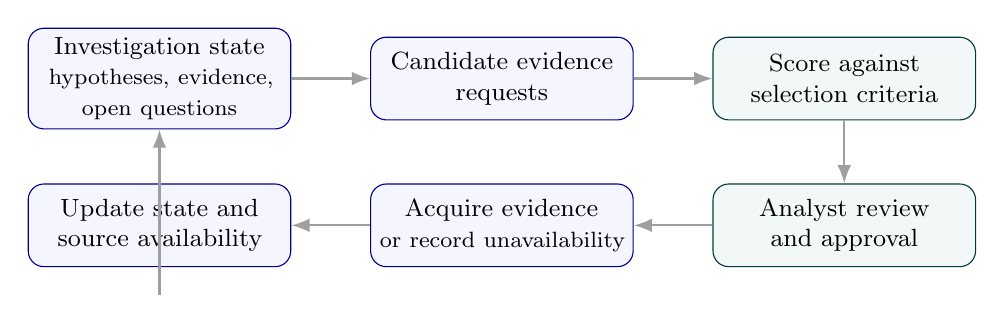
\begin{tikzpicture}[node distance=8mm and 10mm, >=Latex,
  block/.style={draw=blue!55!black, fill=blue!4, rounded corners=2mm, align=center, text width=3.1cm, minimum height=1.05cm, font=\small},
  decision/.style={draw=teal!55!black, fill=teal!5, rounded corners=2mm, align=center, text width=3.1cm, minimum height=1.05cm, font=\small},
  line/.style={->, thick, draw=gray!75}]
\node[block] (state) {Investigation state\\\footnotesize hypotheses, evidence, open questions};
\node[block, right=of state] (candidates) {Candidate evidence\\requests};
\node[decision, right=of candidates] (score) {Score against selection criteria};
\node[decision, below=of score] (review) {Analyst review and approval};
\node[block, left=of review] (acquire) {Acquire evidence\\\footnotesize or record unavailability};
\node[block, left=of acquire] (update) {Update state and source availability};
\draw[line] (state) -- (candidates); \draw[line] (candidates) -- (score);
\draw[line] (score) -- (review); \draw[line] (review) -- (acquire);
\draw[line] (acquire) -- (update);
\draw[line] (update.south) -- ++(0,-0.35) -| ([yshift=-0.35cm]state.south) -- (state.south);
\end{tikzpicture}
\caption{Conceptual adaptive evidence-acquisition loop. The analyst remains in the loop before any request is executed.}
\label{fig:acquisition-loop}
\end{figure}
Figure 1 summarises the loop. The framework is a decision-support component: it recommends requests and qualified conclusions, and an analyst reviews them.
\section{Methodology}
\subsection{Research Design}
The project combines three elements: Design Science Research, prototype development, and controlled experimental evaluation. Design Science Research is appropriate because the contribution is an artefact (a model and policy) intended to address an identified problem, and it requires rigorous evaluation (Hevner et al., 2004). The process follows the activities described by Peffers et al. (2007): problem identification, definition of objectives, design and development, demonstration, evaluation, and communication.
\subsection{Phases}
\begin{enumerate}[leftmargin=*, itemsep=2pt, topsep=3pt]
\item Problem and literature phase: systematic literature search and screening with
documented inclusion criteria, confirmation or revision of the research gap (Section 2), and refinement of requirements.
\item Design phase: specification of the investigation state, availability states, and
selection policy (O1, O2), including documented design alternatives and justification.
\item Prototype phase: implementation of the prototype and the telemetry-degradation
simulator (O3), with versioned code and fixed random seeds.
\item Evaluation phase: controlled experiments, ablations, and analysis (O4).
\item Applicability phase: assessment of Yemen-focused conditions and assumptions
(O5).
\end{enumerate}
\subsection{Prototype Requirements}
The prototype shall (i) maintain the investigation state, (ii) generate and rank candidate requests, (iii) record each answer in one of the three states of Section 4.3, (iv) log all state updates for traceability, and (v) present recommendations to a human reviewer. It shall not execute high-impact actions autonomously.
\subsection{Applicability Assessment}
The Yemen-focused assessment will examine which of the approach’s assumptions (for example availability of logging, query access, analyst capacity, and tooling) hold in the target contexts, and which would need adaptation. Where published evidence is scarce, assumptions will be stated as assumptions, not as established facts about the environment. Any consultation with practitioners will be conducted under the ethical safeguards of Section 8 and subject to institutional approval.
\section{Experimental Evaluation}
\subsection{Compared Methods}
Baseline 1: fixed-priority selection. Candidate requests are taken in a predefined priority order (for example, a playbooklike ordering), without adapting to the evolving state.
Baseline 2: random selection. Candidate requests are chosen uniformly at random among those currently permitted, repeated over many seeds.
Proposed method. The adaptive, cost-aware policy of Section 4.
All methods use the same candidate set, the same belief-update mechanism, and the same investigation budget, so that differences are attributable to the selection policy. Ablated variants of the proposed method (removing, in turn, the cost, delay, availability, and uncertainty components, and the three-state treatment of absence) will quantify each component’s contribution.
\subsection{Metrics}
\begin{table}[htbp]
\centering
\caption{Planned evaluation metrics. Operational definitions will be finalised in the design phase.}
\label{tab:metrics}
\small
\begin{tabularx}{\textwidth}{@{}p{0.23\textwidth}X p{0.13\textwidth}@{}}
\toprule
\textbf{Metric} & \textbf{Intended meaning} & \textbf{Addresses} \\
\midrule
Hypothesis-assessment quality & Agreement of the final hypothesis ranking or assessment with scenario ground truth & RQ3, H1 \\
Investigation cost & Cumulative collection cost, processing cost, and delay consumed & RQ3, H1 \\
Evidence efficiency & Assessment quality or uncertainty reduction obtained per unit cost or per request & RQ3, H2 \\
Uncertainty reduction & Change in uncertainty over hypotheses between start and end of investigation & RQ3, H2 \\
Calibration & Correspondence between stated confidence and observed correctness, using standard calibration measures (Guo et al., 2017) & RQ4 \\
Unsupported-conclusion rate & Share of conclusions not backed by sufficient recorded evidence, including conclusions that rely on absence of evidence alone & RQ4, H3 \\
Robustness & Stability of measures as missing, delayed, or inconsistent telemetry increases & RQ3, H4 \\
Decision traceability & Share of conclusions with a complete chain from request to observation to belief update & RQ1, RQ4 \\
\bottomrule
\end{tabularx}
\end{table}
\subsection{Experimental Procedure and Analysis}
Each scenario is run under each method and each degradation condition with multiple seeds. Comparisons are paired by scenario and condition. Results will be reported with effect sizes and confidence intervals, and significance will be assessed with appropriate nonparametric paired tests or bootstrap procedures, with correction for multiple comparisons. All planned analyses, including those that may disfavour the proposed method, will be
fixed before the final experiments are run. Expected improvements are hypotheses and are not reported as results.
\subsection{Threats to Validity}
Internal validity: shared implementation components may confound policy effects; mitigated by common infrastructure and ablations. Construct validity: metrics are proxies for analyst benefit; traceability and cost measures involve design choices that will be documented. External validity: scenarios and simulated degradation are limited and do not cover all real environments. Ground-truth validity: scenario labels may be incomplete or biased by how scenarios were constructed.
\section{Data, Telemetry Degradation, and Reproducibility}
\subsection{Dataset Selection Criteria}
Candidate datasets and scenarios must: (i) contain multiple telemetry sources with timestamps, so that different evidence requests are meaningful; (ii) provide ground truth sufficient to label hypotheses; (iii) be publicly available or legally and ethically usable for research; (iv) allow evidence requests to be simulated as queries over the data; and (v) be documented well enough to be reproduced. Candidates include the multi-source enterprise event data released by Los Alamos National Laboratory (Kent, 2015); networkflow datasets such as CIC-IDS2017 (Sharafaldin et al., 2018) may serve as a secondary, single-source test, with the limitation that they offer little multi-source structure. If public data lack the required structure, ATT\&CK-aligned scenarios will be constructed on top of them with documented ground truth (Appendix B). Final dataset selection, with justification and known limitations, will be recorded in the design phase.
\subsection{Telemetry Degradation Simulation}
Degradation is applied to the data available to the investigation, not to the ground truth. The simulator is parameterised along four dimensions:
\begin{itemize}[leftmargin=*, itemsep=2pt, topsep=3pt]
\item missing events: removal of events at defined rates and patterns, including whole-source outages;
\item delayed observations: events that become available only after a defined delay;
\item inconsistent source coverage: sources that cover only a subset of assets or periods;
\item access restrictions: sources that cannot be queried, or only at higher cost.
The simulator records which absences are true negatives (the source operated and nothing occurred) and which are coverage gaps, so that the distinction in Section 4.3 can be scored. Degradation levels and patterns will be justified by the missing-data literature (Little and Rubin, 2019) and by documented operational reports, and are fixed in a configuration file.
\end{itemize}
\subsection{Scope of Simulated Limitations}
The simulated limitations are experimental conditions. They do not represent all realworld security environments, and results under them will not be generalised beyond the conditions tested.
\subsection{Reproducibility Procedures}
The project will: publish source code and configuration under version control; fix and report random seeds; record software versions and environment specifications; document dataset versions and preprocessing steps; and release scenario definitions and degradation configurations. Where a dataset’s licence prohibits redistribution, scripts will fetch it from its original source. Reproducibility is bounded by the availability of third-party datasets and by any non-deterministic components; such limits will be reported.
\section{Ethics and Responsible AI}
\begin{itemize}[leftmargin=*, itemsep=2pt, topsep=3pt]
\item Authorised data access: only public datasets, synthetic data, or data for which
explicit authorisation and, where required, institutional ethics approval have been obtained will be used. No system will be accessed or tested without permission.
\item Privacy protection: security telemetry can contain personal data (user identifiers,
addresses, activity traces). Data will be minimised, anonymised or pseudonymised where possible, stored securely, and not redistributed beyond licence terms. Principles of the Menlo Report on ICT research ethics (Dittrich and Kenneally, 2012) guide the work.
\item Responsible security-data handling: no exploit or attack tooling is part of the
contribution; scenario descriptions will remain at a level adequate for evaluation and will not provide operational attack instructions.
\item Human oversight: the system supports analysts and does not make critical security
decisions automatically. Recommendations are advisory, are shown with their evidence chain and uncertainty, and require human review before any request is executed or conclusion is acted upon. This aligns with the emphasis on accountability and transparency in risk-management guidance for AI (National Institute of Standards and Technology, 2023).
\item Transparency about limits: reported results state the conditions under which
they hold, and failures and negative results will be reported.
\end{itemize}
\section{Work Plan, Risks, and Limitations}
\subsection{Work Plan}
\begin{table}[htbp]
\centering
\caption{Proposed work plan. Durations are relative and will be aligned with the programme calendar.}
\label{tab:workplan}
\small
\begin{tabularx}{\textwidth}{@{}p{0.27\textwidth}X p{0.16\textwidth}@{}}
\toprule
\textbf{Phase} & \textbf{Main outputs} & \textbf{Relative timing} \\
\midrule
Problem and literature & Systematic review; confirmed gap; refined requirements & Early \\
Design & Investigation-state model; selection-policy specification & Early--mid \\
Prototype & Prototype; degradation simulator; scenario set & Mid \\
Evaluation & Experiments; ablations; statistical analysis & Mid--late \\
Applicability & Yemen-focused assessment & Late \\
Writing and submission & Thesis, code and data release & Throughout; final \\
\bottomrule
\end{tabularx}
\end{table}
\subsection{Risks and Mitigation}
\begin{itemize}[leftmargin=*, itemsep=2pt, topsep=3pt]
\item No suitable public multi-source dataset: construct documented ATT\&CK-aligned scenarios over available data; state the limitation.
\item Gap already addressed in the literature: the systematic review may show that
the contribution overlaps existing work; the framing would then be revised to a comparison or extension, and the novelty claim withdrawn.
\item Policy offers no advantage over baselines: report the finding; analyse conditions
under which fixed or random selection suffices.
\item Poorly calibrated belief updates: use explicit, auditable updating and calibration
analysis before attributing results to the policy.
\item Limited access to practitioners for the applicability assessment: rely on
literature and documented assumptions, flagged as such.
\end{itemize}
\subsection{Limitations}
The evaluation relies on datasets and simulated degradation and does not establish performance in live operations. Ground truth for hypotheses may be incomplete. The approach concerns evidence selection within an investigation, not detection, and depends on the accuracy of the source registry (coverage, cost, delay). The Yemen-focused assessment will be limited by the availability of published evidence and by access to practitioners. The literature review in this version is preliminary, and the novelty of the contribution is unconfirmed.
\section{Conclusion}
This proposal sets out a plan to study how an investigation can choose its next piece of evidence when telemetry is limited, costly, or unavailable, and how to avoid reading missing data as a finding. It specifies the investigation-state framework, the selection criteria, the baselines and metrics, the simulation of telemetry limitations, and the ethical safeguards. The central claims are hypotheses to be tested, and the stated gap and contributions remain provisional until the systematic literature comparison and the experiments have been completed.
\clearpage
\begin{thebibliography}{99}
\bibitem{ref1} Bushra A. Alahmadi, Louise Axon, and Ivan Martinovic. 99\% false positives: A qualitative study of SOC analysts’ perspectives on security alarms. In 31st USENIX Security Symposium, 2022.
\bibitem{ref2} Douglas G. Altman and J. Martin Bland. Absence of evidence is not evidence of absence. BMJ, 311(7003):485, 1995.
\bibitem{ref3} David Dittrich and Erin Kenneally. The Menlo report: Ethical principles guiding infor- mation and communication technology research. Technical report, U.S. Department of Homeland Security, 2012.
\bibitem{ref4} Finale Doshi-Velez and Been Kim. Towards a rigorous science of interpretable machine learning, 2017.
\bibitem{ref5} Daniel Golovin and Andreas Krause. Adaptive submodularity: Theory and applications in active learning and stochastic optimization. Journal of Artificial Intelligence Research, 42:427–486, 2011.
\bibitem{ref6} Chuan Guo, Geoff Pleiss, Yu Sun, and Kilian Q. Weinberger. On calibration of modern neural networks. In Proceedings of the 34th International Conference on Machine Learning, volume 70 of Proceedings of Machine Learning Research, pages 1321–1330, 2017.
\bibitem{ref7} Wajih Ul Hassan, Shengjian Guo, Ding Li, Zhengzhang Chen, Kangkook Jee, Zhichun Li, and Adam Bates. NoDoze: Combatting threat alert fatigue with automated provenance triage. In Network and Distributed System Security Symposium (NDSS), 2019.
\bibitem{ref8} Alan R. Hevner, Salvatore T. March, Jinsoo Park, and Sudha Ram. Design science in information systems research. MIS Quarterly, 28(1):75–105, 2004.
\bibitem{ref9} Grant Ho, Mayank Dhiman, Devdatta Akhawe, Vern Paxson, Stefan Savage, Geoffrey M. Voelker, and David Wagner. Hopper: Modeling and detecting lateral movement. In 30th USENIX Security Symposium, 2021.
\bibitem{ref10} Md Nahid Hossain, Sadegh M. Milajerdi, Junao Wang, Birhanu Eshete, Rigel Gjomemo, R. Sekar, Scott D. Stoller, and V. N. Venkatakrishnan. SLEUTH: Real-time attack scenario reconstruction from COTS audit data. In 26th USENIX Security Symposium, 2017.
\bibitem{ref11} Ronald A. Howard. Information value theory. IEEE Transactions on Systems Science and Cybernetics, 2(1):22–26, 1966.
\bibitem{ref12} Eyke Hüllermeier and Willem Waegeman. Aleatoric and epistemic uncertainty in machine learning: An introduction to concepts and methods. Machine Learning, 110(3):457–506, 2021.
\bibitem{ref13} Leslie Pack Kaelbling, Michael L. Littman, and Anthony R. Cassandra. Planning and acting in partially observable stochastic domains. Artificial Intelligence, 101(1–2):99–134, 1998.
\bibitem{ref14} Alex Kendall and Yarin Gal. What uncertainties do we need in Bayesian deep learning for computer vision? In Advances in Neural Information Processing Systems 30, 2017.
\bibitem{ref15} Alexander D. Kent. Comprehensive, multi-source cyber-security events. Los Alamos National Laboratory dataset, 2015.
\bibitem{ref16} Karen Kent and Murugiah Souppaya. Guide to computer security log management. Special Publication 800-92, National Institute of Standards and Technology, 2006.
\bibitem{ref17} Faris Bugra Kokulu, Ananta Soneji, Tiffany Bao, Yan Shoshitaishvili, Ziming Zhao, Adam Doupé, and Gail-Joon Ahn. Matched and mismatched SOCs: A qualitative study on security operations center issues. In Proceedings of the ACM SIGSAC Conference on Computer and Communications Security (CCS), 2019.
\bibitem{ref18} Andreas Krause and Carlos Guestrin. Optimal value of information in graphical models. Journal of Artificial Intelligence Research, 35:557–591, 2009.
\bibitem{ref19} Robert M. Lee and David Bianco. Generating hypotheses for successful threat hunting. White paper, SANS Institute, 2016.
\bibitem{ref20} Roderick J. A. Little and Donald B. Rubin. Statistical Analysis with Missing Data. Wiley, 3rd edition, 2019.
\bibitem{ref21} Scott M. Lundberg and Su-In Lee. A unified approach to interpreting model predictions. In Advances in Neural Information Processing Systems 30, 2017.
\bibitem{ref22} Sadegh M. Milajerdi, Rigel Gjomemo, Birhanu Eshete, R. Sekar, and V. N. Venkatakrishnan. HOLMES: Real-time APT detection through correlation of suspicious information flows. In IEEE Symposium on Security and Privacy, 2019.
\bibitem{ref23} National Institute of Standards and Technology. Artificial intelligence risk management framework (AI RMF 1.0). NIST AI 100-1, NIST, 2023.
\bibitem{ref24} Ken Peffers, Tuure Tuunanen, Marcus A. Rothenberger, and Samir Chatterjee. A design science research methodology for information systems research. Journal of Management Information Systems, 24(3):45–77, 2007.
\bibitem{ref25} Burr Settles. Active learning literature survey. Computer Sciences Technical Report 1648, University of Wisconsin–Madison, 2009.
\bibitem{ref26} Iman Sharafaldin, Arash Habibi Lashkari, and Ali A. Ghorbani. Toward generating a new intrusion detection dataset and intrusion traffic characterization. In Proceedings of the 4th International Conference on Information Systems Security and Privacy (ICISSP), 2018.
\bibitem{ref27} Blake E. Strom, Andy Applebaum, Doug P. Miller, Kathryn C. Nickels, Adam G. Pen- nington, and Cody B. Thomas. MITRE ATT\&CK: Design and philosophy. Technical report, The MITRE Corporation, 2018.
\bibitem{ref28} Richard S. Sutton and Andrew G. Barto. Reinforcement Learning: An Introduction. MIT Press, 2nd edition, 2018.
\end{thebibliography}
\appendix
\section{Working Terminology}
\paragraph{Telemetry} Records produced by monitored systems (for example authentication, process, network, and DNS logs) that can be queried during an investigation.
\paragraph{Evidence of absence} A verified negative: a source with adequate coverage confirms the event did not occur.
\paragraph{Absence of evidence} No usable record because data were unavailable, incomplete, delayed, or outside coverage; the question remains unresolved.
\paragraph{Evidence request} A query or collection action against a telemetry source.
\paragraph{Investigation state} The current hypotheses, observations, unresolved questions, and source registry.
\paragraph{Unsupported conclusion} A conclusion not backed by sufficient recorded evidence, including one resting on absence of evidence alone.
\section{Scenario Specification Template}
Each evaluation scenario will be documented with the following fields:
\begin{itemize}[leftmargin=*,itemsep=2pt]
\item Scenario identifier and source dataset (with version).
\item Ground-truth hypotheses and, where applicable, the corresponding ATT\&CK techniques.
\item Telemetry sources available and their coverage, cost, delay, and access status.
\item Candidate evidence requests and the questions they address.
\item Degradation configuration (missing, delayed, inconsistent, restricted) and seed.
\item List of absences labelled as true negatives or coverage gaps.
\item Criteria used to label hypothesis outcomes.
\end{itemize}
\end{document}
